\documentclass[tikz,border=4pt]{standalone}

\usepackage{amsmath,bm}
\usetikzlibrary{positioning,arrows.meta}

\tikzset{font=\sffamily}

\begin{document}
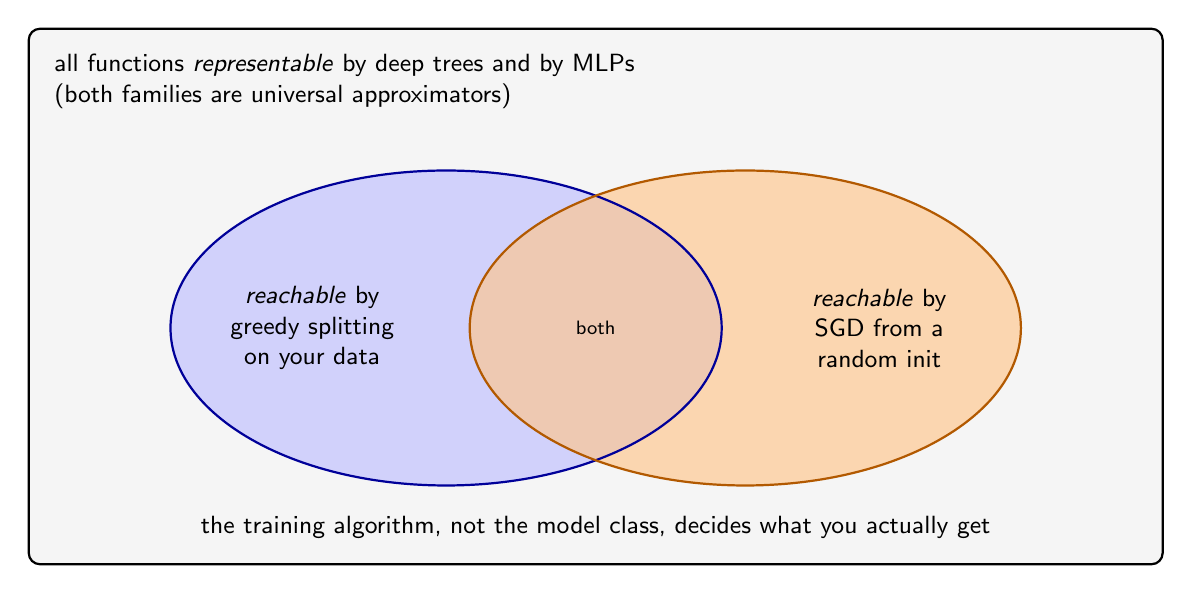
\begin{tikzpicture}[x=1cm, y=1cm]
  \draw[rounded corners, thick, fill=gray!8] (-7.2, -3.4) rectangle (7.2, 3.4);
  \node[font=\sffamily\small, anchor=north west, align=left] at (-7.0, 3.2)
    {all functions \emph{representable} by deep trees and by MLPs\\(both families are universal approximators)};

  \fill[blue!25, opacity=.65]   (-1.9, -0.4) ellipse (3.5 and 2.0);
  \fill[orange!45, opacity=.65] (1.9, -0.4) ellipse (3.5 and 2.0);
  \draw[blue!60!black, thick]   (-1.9, -0.4) ellipse (3.5 and 2.0);
  \draw[orange!70!black, thick] (1.9, -0.4) ellipse (3.5 and 2.0);

  \node[font=\sffamily\small, align=center] at (-3.6, -0.4)
    {\emph{reachable} by\\greedy splitting\\on your data};
  \node[font=\sffamily\small, align=center] at (3.6, -0.4)
    {\emph{reachable} by\\SGD from a\\random init};
  \node[font=\sffamily\scriptsize, align=center] at (0, -0.4) {both};

  \node[font=\sffamily\small, anchor=south, align=center] at (0, -3.2)
    {the training algorithm, not the model class, decides what you actually get};
\end{tikzpicture}
\end{document}
